
% !TeX program = xelatex
% !TEX root = main.tex
% !TeX encoding = UTF-8
\documentclass[10.5pt,compsoc]{CjC}
%\usepackage{CJKutf8}
%\usepackage{CJK}
\usepackage{graphicx}
\usepackage{footmisc}
\usepackage{subfigure}
\usepackage{url}
\usepackage{multirow}
\usepackage{algorithm}
\usepackage{algorithmic}
\usepackage{algpseudocode}
\renewcommand{\algorithmicrequire}{ \textbf{Input:}}
\renewcommand{\algorithmicensure}{ \textbf{Output:}}
\usepackage[noadjust]{cite}
\usepackage{amsmath,amsthm}
\usepackage{amssymb,amsfonts}
\usepackage{booktabs}
\usepackage{color}
\usepackage{ccaption}
\usepackage{booktabs}
\usepackage{float}
\usepackage{fancyhdr}
\usepackage{caption}
\usepackage{xcolor,stfloats}
\usepackage{comment}
\setcounter{page}{1}
\graphicspath{{figures/}}
\usepackage{cuted}%flushend,
\usepackage{captionhack}
\usepackage{epstopdf}
%\usepackage{ccmap}
%\CJKtilde
%\usepackage{CJKpunct} 
%\usepackage[lite,subscriptcorrection,slantedGreek,nofontinfo]{mtpro2}

%===============================%

%\firstfootname{ \quad \quad }

%footnote use of *
\renewcommand{\thefootnote}{\fnsymbol{footnote}}
\setcounter{footnote}{0}
\renewcommand\footnotelayout{\zihao{5-}}

\newtheoremstyle{mystyle}{0pt}{0pt}{\normalfont}{1em}{\bf}{}{1em}{}
\theoremstyle{mystyle}
\renewcommand\figurename{figure~}
\renewcommand{\thesubfigure}{(\alph{subfigure})}
\newcommand{\upcite}[1]{\textsuperscript{\cite{#1}}}
\renewcommand{\labelenumi}{(\arabic{enumi})}
\newcommand{\tabincell}[2]{\begin{tabular}{@{}#1@{}}#2\end{tabular}}
\newcommand{\abc}{\color{white}\vrule width 2pt}
\makeatletter
\renewcommand{\@biblabel}[1]{[#1]\hfill}
\makeatother
\setlength\parindent{2em}
%\renewcommand{\hth}{\heiti }
%\renewcommand{\htss}{\begin{CJK*}{UTF8}{song}}


\begin{document}
\hyphenpenalty=50000
\makeatletter
\newcommand\mysmall{\@setfontsize\mysmall{7}{9.5}}
\newenvironment{tablehere}
  {\def\@captype{table}}

\let\temp\footnote
\renewcommand \footnote[1]{\temp{\zihao{-5}#1}}


\thispagestyle{plain}%
\thispagestyle{empty}%
\pagestyle{CjCheadings}

\begin{table*}[!t]
\vspace {-13mm}


\centering
\vspace{11mm}
\heiti  
{\zihao{2} 周泽人第三次作业Latex2}

\vskip 5mm

{\zihao{3} \fangsong 
周泽人$^{1)}$\quad  214712279 \quad 
 }

\vspace{5mm}
\zihao{6}{\songti 
$^{1)}$中南大学 计算机学院, 长沙市 中国 410000)
 }

\end{table*}  


\begin{table}
\centering
\caption{周泽人214712279}
\label{table-sample}
\begin{tabular}{|p{5.1em}|r|r|r}
\hline
name & class & id \\
\hline
zhouzeren & 1 & 214712279 \\
\hline
\end{tabular}
\end{table}

\begin{figure}[H]
\centering
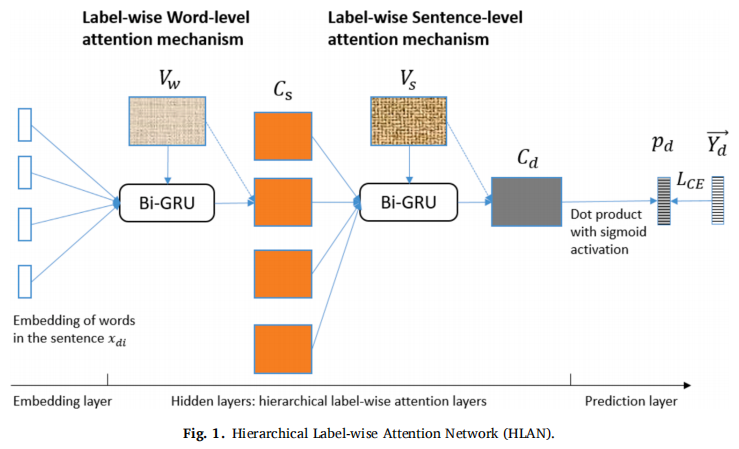
\includegraphics[width=5.6cm]{test.png}
\caption{test figure}
\label{test-figure}
\end{figure}


\begin{algorithm}[H]
\caption{algorithm} 
\hspace*{0.02in} {\bf Input:}
input parameters A\\
\hspace*{0.02in} {\bf Output:} 
output result
\begin{algorithmic}[1]
\For{condition} 
  \State ...
  \If{condition}
    \State ...
  \Else
    \State ...
  \EndIf
\EndFor
\State \Return result
\end{algorithmic}
\end{algorithm}

\begin{thebibliography}{00}
\bibitem{b1} T. Baumel, J. Nassour-Kassis, R. Cohen, M. Elhadad, N. Elhadad, Multi-label classification of patient notes: case study on ICD code assignment, in: Workshops at the Thirty-Second AAAI Conference on Artificial Intelligence, 2018, pp. 409–416.
\end{thebibliography}


\end{document}

